\documentclass[]{article}

\usepackage[T1]{fontenc}
\usepackage[utf8]{inputenc}
\usepackage{polski}
\usepackage{url}
\usepackage{graphicx}
\usepackage[section]{placeins}

\title{Specyfikacja funkcjonalna\\Projekt zespołowy\\Optymalizacja przewozu pacjentów}
\author{Bartłomiej Łukasik\\Damian Wróblewski\\Karol Kociołek}

\begin{document}

\maketitle

\section{Cel projektu}
Program po dostarczeniu danych:
\begin{itemize}
\item interaktywnie wyświetla trasy pacjentów
\item stworzy listy przewozów wszystkich pacjentów
\item wizualizacja mapy na podstawie danych wejściowych o konturze wielościanu wypukłego 
\end {itemize}


\section{Scenariusz użycia}
\begin {enumerate}
\item Przygotowanie odpowiedniego pliku z danymi
\item Uruchomienie programu
\item Przekazanie pliku do programu przez GUI (plik dotyczący opisu mapy)
\item (opcjonalnie) Przekazanie plików z pacjentami (maks 5)
\item (opcjonalnie) Dodanie pacjentów z poziomu GUI
\item Symulacja tras
\item Otrzymanie pliku z danymi wyjściowymi
\item Program kończy prace\\
\end {enumerate}
\clearpage

\section{Ekran działania programu}

\begin{figure}[!htb]
\resizebox{14cm}{!}{
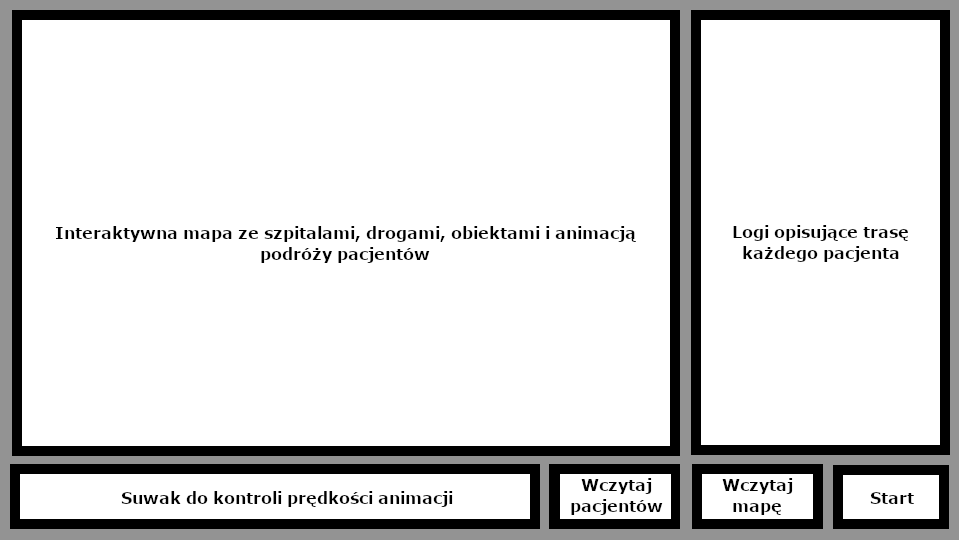
\includegraphics{Ekran_dzialania.png}
}
\end{figure}



\section{Opis pliku wejściowego}
Nazwa pliku podawana jest podczas uruchamiania programu.
Plik powinień być w formacie tekstowym o rozszerzeniu ".txt". \\
Zawiera on 3 sekcje (pierwsza linia to tytuł następne to dane) w kolejności:
\begin{itemize}
\item Szpitale (id | nazwa | wsp. x | wsp. y | Liczba łóżek | Liczba wolnych łóżek)
\item Obiekty (id | nazwa | wsp. x | wsp. y)
\item Drogi (id | idszpitala | idszpitala | odległość)
\end{itemize}
Każda sekcja zawiera w pierwszej lini tytuł i w każdej następnej dane(nowa sekcja rozpoczyna się od nowej lini pod danych)\\
\\
Format tytułu:\\
Pierwszy znak to: "\#"\\
Następnie nazwa i w nawiasie nazwy kolumn w kolejności w jakiej występują elementy obiektów\\
\\
Format danych:\\
Wypisywane są po jednym obiekcie w jednej lini\\
Każdy obiekt składa się z kilku elementów odzielonych znakiem "|"\\
Z jakich elemntów składa się obiekt w sekcji zaprezentowane jest wyżej w nazwach sekcji\\
\\
Przykład pliku:\\
\\
\# Szpitale (id | nazwa | wsp. x | wsp. y | Liczba łóżek | Liczba wolnych łóżek)\\
1 | Szpital Wojewódzki nr 997 | 10 | 10 | 1000 | 100\\
2 | Krakowski Szpital Kliniczny | 100 | 120 | 999 | 99\\
3 | Pierwszy Szpital im. Prezesa RP | 120 | 130 | 99 | 0\\
4 | Drugi Szpital im. Naczelnika RP | 10 | 140 | 70 | 1\\
5 | Trzeci Szpital im. Króla RP | 140 | 10 | 996 | 0\\
\# Obiekty (id | nazwa | wsp. x | wsp. y)\\
1 | Pomnik Wikipedii | -1 | 50\\
2 | Pomnik Fryderyka Chopina | 110 | 55\\
3 | Pomnik Anonimowego Przechodnia | 40 | 70\\
\# Drogi (id | idszpitala | idszpitala | odległość)\\
1 | 1 | 2 | 700\\
2 | 1 | 4 | 550\\
3 | 1 | 5 | 800\\
4 | 2 | 3 | 300\\
5 | 2 | 4 | 550\\
6 | 3 | 5 | 600\\
7 | 4 | 5 | 750\\

\section{Opis pliku wyjściowego}
Na wyjściu program zwraca plik o nazwie "wynik.txt" z listą pacjentów i ich trasą\\
Przykład pliku:\\
1    ->  Krakowski Szpital Kliniczny - Pierwszy Szpital im. Prezesa RP\\
...\\


\section{Błędy}
W przypadku niepoprawnych danych wiejściowych program zwróci komunikat z opisem błędu

\end{document}